%!TEX root = main.tex
\section{User Study Evaluation\label{sec:userstudy}}
\subsection{Methods}
We evaluate the utility of \system by performing a between-subject user study focusing on addressing the following research questions:
\begin{denselist}
	\item RQ1: How \textit{interesting} are the visualizations in the dashboard perceived subjectively by the users?
	\item RQ2: How well do the dashboards \textit{summarize} the relative importance of different attributes within a given dataset?
	\item RQ3: How \textit{informative} are the visualizations in the dashboard at providing users with an accurate understanding for unseen child visualizations? %effective is our tool at guiding users towards safe and informative visualization references? 
	% in providing analysts with task-specific insights? (including identifying important features for prediction tasks and estimating the distribution of an unseen visualization)
	% \item RQ3: How useful are the visualizations in the recommended dashboard to analysts?
\end{denselist}
We recruited 18 participants with prior experience in working with data. Participants included undergraduate and graduate students, researchers, and data scientists, with 1 to 14 years of data analysis experience (average = 5.61).  %This can include, but are not limited to, browsing and reading data, data cleaning and wrangling, data visualization and model building. The inclusion criteria is assessed based on a self-reporting basis in the pre-study survey.
%an average of 5.61 years of experience working with data.
There were 8 female and 10 male participants. No participants reported prior experience in working with the two datasets used in the study. Participants were randomly assigned two of the three dashboards with k=10 visualizations generated by following conditions. 
\stitle{\system:} The dashboards for this condition are generated by the frontier greedy algorithm (described in Section \ref{sec:algorithms}) and displayed in a hierarchical layout (as seen in Figure~\ref{fig:overview}). In order to establish a fair comparison with the two other conditions, we deactivated the interactive node expansion capabilities.
\stitle{\BFS:} Starting from the visualization of the entire population, $k$ visualizations is selected level-wise, traversing down the subset lattice, adding the visualizations at the first level with 1-filter combination one at a time, proceeding with the 2-, 3-, and so on, until $k$ visualizations have been added to the dashboard. This baseline is designed to simulate the dashboard generated by a meticulous analyst who exhaustively inspects all possible visualization combinations from the top-down. The chosen visualizations are displayed in a 5x2 table layout in the traversed order.
\stitle{\cluster:} K-Means clustering is performed on the dataset with $k$ clusters, corresponding to $k$, the number of visualizations to be shown in the dashboard. For each representative cluster, we select the visualization with the least number of filter conditions for interpretability\footnote{Due to this requirement, the overall visualization is guaranteed to be picked as one of the displayed visualizations.} and display them in a 5x2 table layout. This baseline is designed to showcase a diverse set of pattern distributions within the dataset.
\par Each participant were assigned two different conditions on two different datasets. The ordering of each condition was randomized to prevent confounding learning effects.%We randomize the ordering for each task combination to prevent confounding learning effects. 
The study began with a 5 minute tutorial using dashboards generated from the Titanic dataset~\cite{titanic} for each condition. To prevent bias across conditions, participants were not provided an explanation of how the dashboard was generated and why the visualizations were arranged in a particular way. Then, participants proceeded onto the Police Stop dataset, as described in Section~\ref{sec:system}.%, which contains visualizations of the \% of police stop that resulted in a warning, ticket, or an arrest.
%, which contains a total of 312948 records of vehicle and pedestrian stops from law enforcement departments in Connecticut, dated from 2013 to 2015. 
We generated dashboards of bar chart visualizations with x-axis as the stop outcome (i.e., whether the police stop resulted in a ticket, warning, or arrest) and y-axis as the percentage of police stops that led to each outcome. \techreport{The attributes in the dataset include driver gender, age, race, and the stop time of day, whether a search was conducted, and whether contraband was found.}
\par The second dataset in the study is the Autism dataset~\cite{autism}, which includes the result of autism spectrum disorder screening for 704 adults. The attributes in the dataset are binary responses to 10 diagnostic questions that are part of the screening process. This dataset serves as a data-agnostic condition, since there was no descriptions of the questions or answer labels provided to the user. We generate dashboard visualizations based on whether the participant is diagnosed with autism or not. 
\par Participants were given some time to read through a worksheet containing the descriptions of the data attributes. Then, they were given an attention check question where they were given a verbal description of the visualization filter and asked about the distributions for the corresponding visualization in the dashboard. After understanding the dataset and chart schema, participants were asked to accomplish the following tasks in the prescribed order below:
\stitle{Retrieval:} Participants were asked to talk aloud as they interpreted the visualizations in the dashboard and mark each visualization as either interesting, not interesting, or leave it as unselected. This task was intended to measure how interesting are the selected visualizations to participants (RQ1).%well are participants at retrieving interesting visualizations (RQ1).

\stitle{Attribute Ranking:} Participants were given a sheet of paper with all the attributes listed and asked to rank the attributes in order of importance in contributing to a particular outcome (e.g., factors leading to an arrest or autism diagnosis). Participants were allowed to assign equal ranks to more than one attributes or skip attributes that they were unable to infer their importance for. Attribute ranking tasks are common in feature selection and other data science tasks. The goal of this task is to measure how well participants understand the relative importance of each attribute in contributing towards an outcome (RQ2).

\stitle{Prediction:} Participants were given a separate worksheet and asked to sketch an estimate for a visualization that is not present in the dashboard. For every condition, the visualization to be estimated contained 2 filter combinations, with exactly one parent present in the given dashboard. After making the prediction, participants were shown the actual data distribution and asked to rate on a Likert scale of 10 how surprising the result was (where 1 is not surprising and 10 is very surprising). The prediction task measures how accurate participants are at predicting an unseen visualization, estimating how well they understood key informative insights that influences other distributions from the dataset(RQ3).
% \stitle{Deep Prediction:} This task is similar to the shallow prediction, except that the visualization to be estimated is ``deep'' in the sense that it has 3 filter combinations, with only one parent in the given dashboard. Both prediction tasks measure how accurate participants are at predicting an unseen visualization (RQ3).
\par We repeat the same study procedure described above for the Autism dataset. At the end of the study, we asked two open-ended questions regarding the stories and insights that they have learned and what they like or dislike about each dashboard. On average, the study lasted around 48 minutes.
%The user study is composed of two phases. Phase one of the experiment focuses on comparing our tool against a set of baselines intended to simulate the natural sequence of visualizations that an analyst would encounter through various approaches during exploratory analysis. The baselines include:
%To prevent learning effects, the ordering of the baselines will be randomized across users.
% \par At the beginning of the study, participants were provided with a dashboard from an example dataset, as well as an explanation of how the dashboard is generated. For each of the visualization dashboard, participants are asked to mark visualizations as interesting/not interesting while explaining their reasoning for each annotation. Then, they are asked to summarize a list of insights that they have discovered after browsing through all visualizations in the dashboard. Participants also answer a set of task-specific questions related to causality and outliers[?], in the form as shown in the example [*]. These tasks are repeated for all baselines and our tool in randomized order on different datasets to prevent learning effects. At the end of phase one, participants are asked to comment on their experiences with each method, as well as the pros and cons of each of the tools. This phase of the experiment is designed to quantify the effects of RQ 1 and 2. In the end, we ask participants to discuss the interesting insights drawn from looking at the recommended dashboards as well as  ------.
%\par To prevent fatigue, after a 5 minute break, the participants then proceed onto phase two of the study, where they are given [10] dashboards generated by our tool and are asked to engage in a talk-aloud exercise as they browse the recommended visualizations. This is a more open-ended study intended for addressing RQ3 that can reveal our tool show unimportant results across different datasets and/or highlight larger selection of the types of insights that can be generated from the tool.
\subsection{Quantitative Results}
% In order to evaluate the efficacy of our system against the two baselines, we will first examine the quantitative results to address RQ1 and RQ2 and then discuss the qualitative findings to address RQ3.
%\dor{In general, we might have to make better connection between the RQs and the study results.}
\stitle{Retrieval (RQ1):} Using the click-stream data logged from the user study, we recorded whether a participant marked a visualization in the dashboard as interesting, not interesting, or left the visualization unselected. %Since we do not have objective ground truths of which visualization is interesting or not, we use the participant's consensus to come up with a score for each visualization. In this scoring scheme, if visualization is marked as interesting, that visualization receives a score of 1; if a visualization is marked as uninteresting, the visualization incurs a penalty of -0.5\footnote{The reason why we chose a lower penalty score for disinterested clicks than the interested click reward is that some of the participants did not chose to mark visualizations that they thought were uninteresting as disinterested explicitly and chose to simply keep them unselected.}; no score is assigned if the visualization is unselected, then the scores are summed over all users who have seen the visualization. Each user is then assigned a score based on the product of their retrieval score and the consensus score (i.e. user would receive a higher score if selected visualization was highly ranked by consensus).
% Since interestingness is a subjective measure, 
% %Since we do not have a objective ground truth on which visualization is interesting or not interesting, 
% we devise a popularity-based metric that measures how interesting a visualization is amongst all participants. We assign the selection made by user j to visualization i with score $\delta_{ij}$ of 1 if a user is interested, 0 if they leave it unselected, and -1 if they are not interested. 
% %Here i indexes the visualization and j indexes the user. 
% % As shown in Equation~\ref{weighting}, w
% % \begin{equation}\label{weighting}
% % 	\delta_{ij}= \left\{\begin{matrix}
% % 	 1& \textrm{interested}
% % 	\\ 0 & \textrm{unselected}
% % 	\\ -1 & \textrm{not interested}
% % 	\end{matrix}\right.
% % \end{equation}
% We obtain a consensus score for each visualization to measure how frequently the visualization is regarded as interesting by summing over all users' vote on that visualization.
% \begin{equation}\label{vote}
% \textrm{consensus}(V_i) =\sum_{j\in user} \delta_{ij}
% \end{equation}
% Given a consensus measure of how interesting a visualization is, we can define a rating score which measures how good a particular user's rating is, by taking the product of the consensus interestingness score and the rating value, as shown in Equation \ref{rank}. Intuitively, a rating should be rewarded more if it has retrieved interesting visualization agreed by many other users, likewise, ratings that does not retrieve such visualizations should be penalized more heavily.
% describes how the rating score (which measures how good the user's particular rating is) is the product of consensus score (how frequently is a visualization regarded as interesting?) and the rated value ($\delta_{ij}$).
% \begin{equation}\label{rank}
% \textrm{rating score}(V_{ij}) =\textrm{consensus}(V_i) \cdot \delta_{ij}
% \end{equation}
Table~\ref{table:interestingScore} summarizes counts of visualizations marked as interesting or not interesting aggregated across conditions. We also normalize the interesting count by the total number of selected visualizations to account for variations in how some participants select more visualizations than others. The result indicate that participants who used \system\ found more visualizations that they found interesting compared to the \BFS  and \cluster condition.
\begin{table}[ht!]
	\centering
	\begin{tabular}{lrrr}
	\hline
	 Condition             &   Storyboard &   BFS &   Cluster \\
	\hline
	 Interesting            &  \cellcolor{blue!25}       66    & 61    &      51   \\
	 Not Interesting        &  \cellcolor{blue!25}       10    & 20    &      22   \\
	 Interesting (Normalized) &   \cellcolor{blue!25}       0.87 &  0.75 &       0.7 \\
	\hline
	\end{tabular}
	\caption{Total count of visualizations marked as interesting or not interesting across the different algorithms. \system leads to more visualizations marked as interesting and fewer visualizations marked as uninteresting.}
	\label{table:interestingScore}
	\vspace{-20pt}
\end{table}
% \begin{table}[ht!]
% 	\centering
% 	\begin{tabular}{lrrr}
% 		\hline
% 		 Dataset   &   \system &   Cluster &   BFS \\
% 		\hline
% 		 Police    &      1.03 &      0.87 &  1.65 \\
% 		 Autism    &      3.55 &      3.00 &  1.90 \\
% 		\hline
% 	\end{tabular}
% 	\caption{Average consensus-agreement score for different algorithm and datasets.}%\agp{breakdown by interested and not interested}}
% 	\label{table:interestingScore}
% 	\vspace{-20pt}
% \end{table}
% \dor{We should consider doing a Chi square rather than averaging here to show significant difference between groups.}
%Even though participants were asked to --- daily experiences to answer the question, b
% \npar Due to the highly subjective nature of the retrieval task, the interestingness selection for the Police dataset was biased by participant's priors and intuition about the attributes. For example, while all participants who have seen the visualization "duration=30+min" verbally noted that stop duration is a crucial factor that leads to arrest, only 4 users marked it as interesting. 5 participants marked the visualization as not interesting and 4 left it unselected, because the visualization was not very surprising as it agreed with their intuition that ``\textit{if the police stop is taking a long time, something has probably gone wrong}''.
% \par Since the attributes in the Autism dataset are simply question numbers, participants could not associate any priors to their interestingness selection. In this prior-agnostic case, participants who used \system\ found more visualizations of interest that corresponded to the consensus, indicating that there are more interesting visualizations picked out by \system\ than compared to \BFS (p=0.003) and \cluster (p=0.09).

\stitle{Attribute Ranking (RQ2):}
To determine the attribute importance for a dataset, we computed the Cramer's V statistics between attributes to be ranked and the attributes of interest. Cramer's V test makes use of the chi-square statistics to determine the strength of association between attributes~\cite{McHugh2013}. Using the ground truth based on ranks determined by Cramer's V statistics, we compute the normalized discounted cumulative gain (NDCG@k) of each participant's ranking average over all tasks\footnote{Since participants are asked to examine all attributes, the k for NDCG@k corresponds to total number of attributes in that dataset.}, as detailed in Table \ref{table:ndcgRankingResult}.
\begin{table}[ht!]
	\centering
	\begin{tabular}{lrrr}
	\hline
	 Dataset   &   \system &  \BFS &  \cluster   \\
	\hline
	 Police    &      0.63 &       \cellcolor{blue!25}0.84 &  0.45 \\
	 Autism    &      \cellcolor{blue!25}0.50 &       0.24&0.30   \\
	\hline
	\label{table:ndcg_ranking_result}
	\end{tabular}
	\caption{NDCG@10 scores for the attribute ranking task.}
	\vspace{-20pt}
    \label{table:ndcgRankingResult}
\end{table}
We see that \system\ performs better than clustering in both cases. Since clustering seeks visualizations that exhibit diversity in the shape of the data distribution, it results in visualizations with many filter combinations, which is hard to interpret without appropriate context to compare against. \BFS performs better than \system in the Police dataset, but not in the Autism dataset. \BFS may have performed better than \system\ in the Police dataset for a combination of two reasons: 1) since \BFS exhaustively displays all attributes sequentially, for the Police dataset it happened to select several of the important attributes (related to contraband and search) to display in the first 10 visualizations and 2) some participants had priors on the data attribute which influenced their ranking. However, with a budget of k=10, only visualizations regarding diagnostic questions 1-5 fit in the dashboard for the Autism dataset, so the poor ranking behavior comes from the fact that the \BFS generated dashboard failed to display the important attributes (questions 6 and 9) given the limited budget. This demonstrates \BFS's lack of providing a guarantee especially when exhaustive exploration has a limit (e.g., time or attention of analyst). In general, our results indicate that using \system, users gain a better understanding of attribute influence and importance.
\stitle{Prediction (RQ3):} In order to compare how accurate analysts' mental model for various ---drill down paths for investigating RQ3, we use the prediction tasks as a proxy for how informative the selected visualizations in the dashboard are. Informativeness is measured by how accurate participants are at predicting an unseen visualization. In order to measure how accurate participants' decisions are, we computed the Euclidean distance between their predicted distributions and ground truth data distributions. As shown in Figure \ref{fig:distance}, the predictions made by using \system\ is closer to the actual distribution compared to the baselines. This indicates that users are able to more accurately reason about how unseen data would behave with \system. \agp{Why was cluster better in one setting but not the other?}
\begin{figure}[h!]
\centering
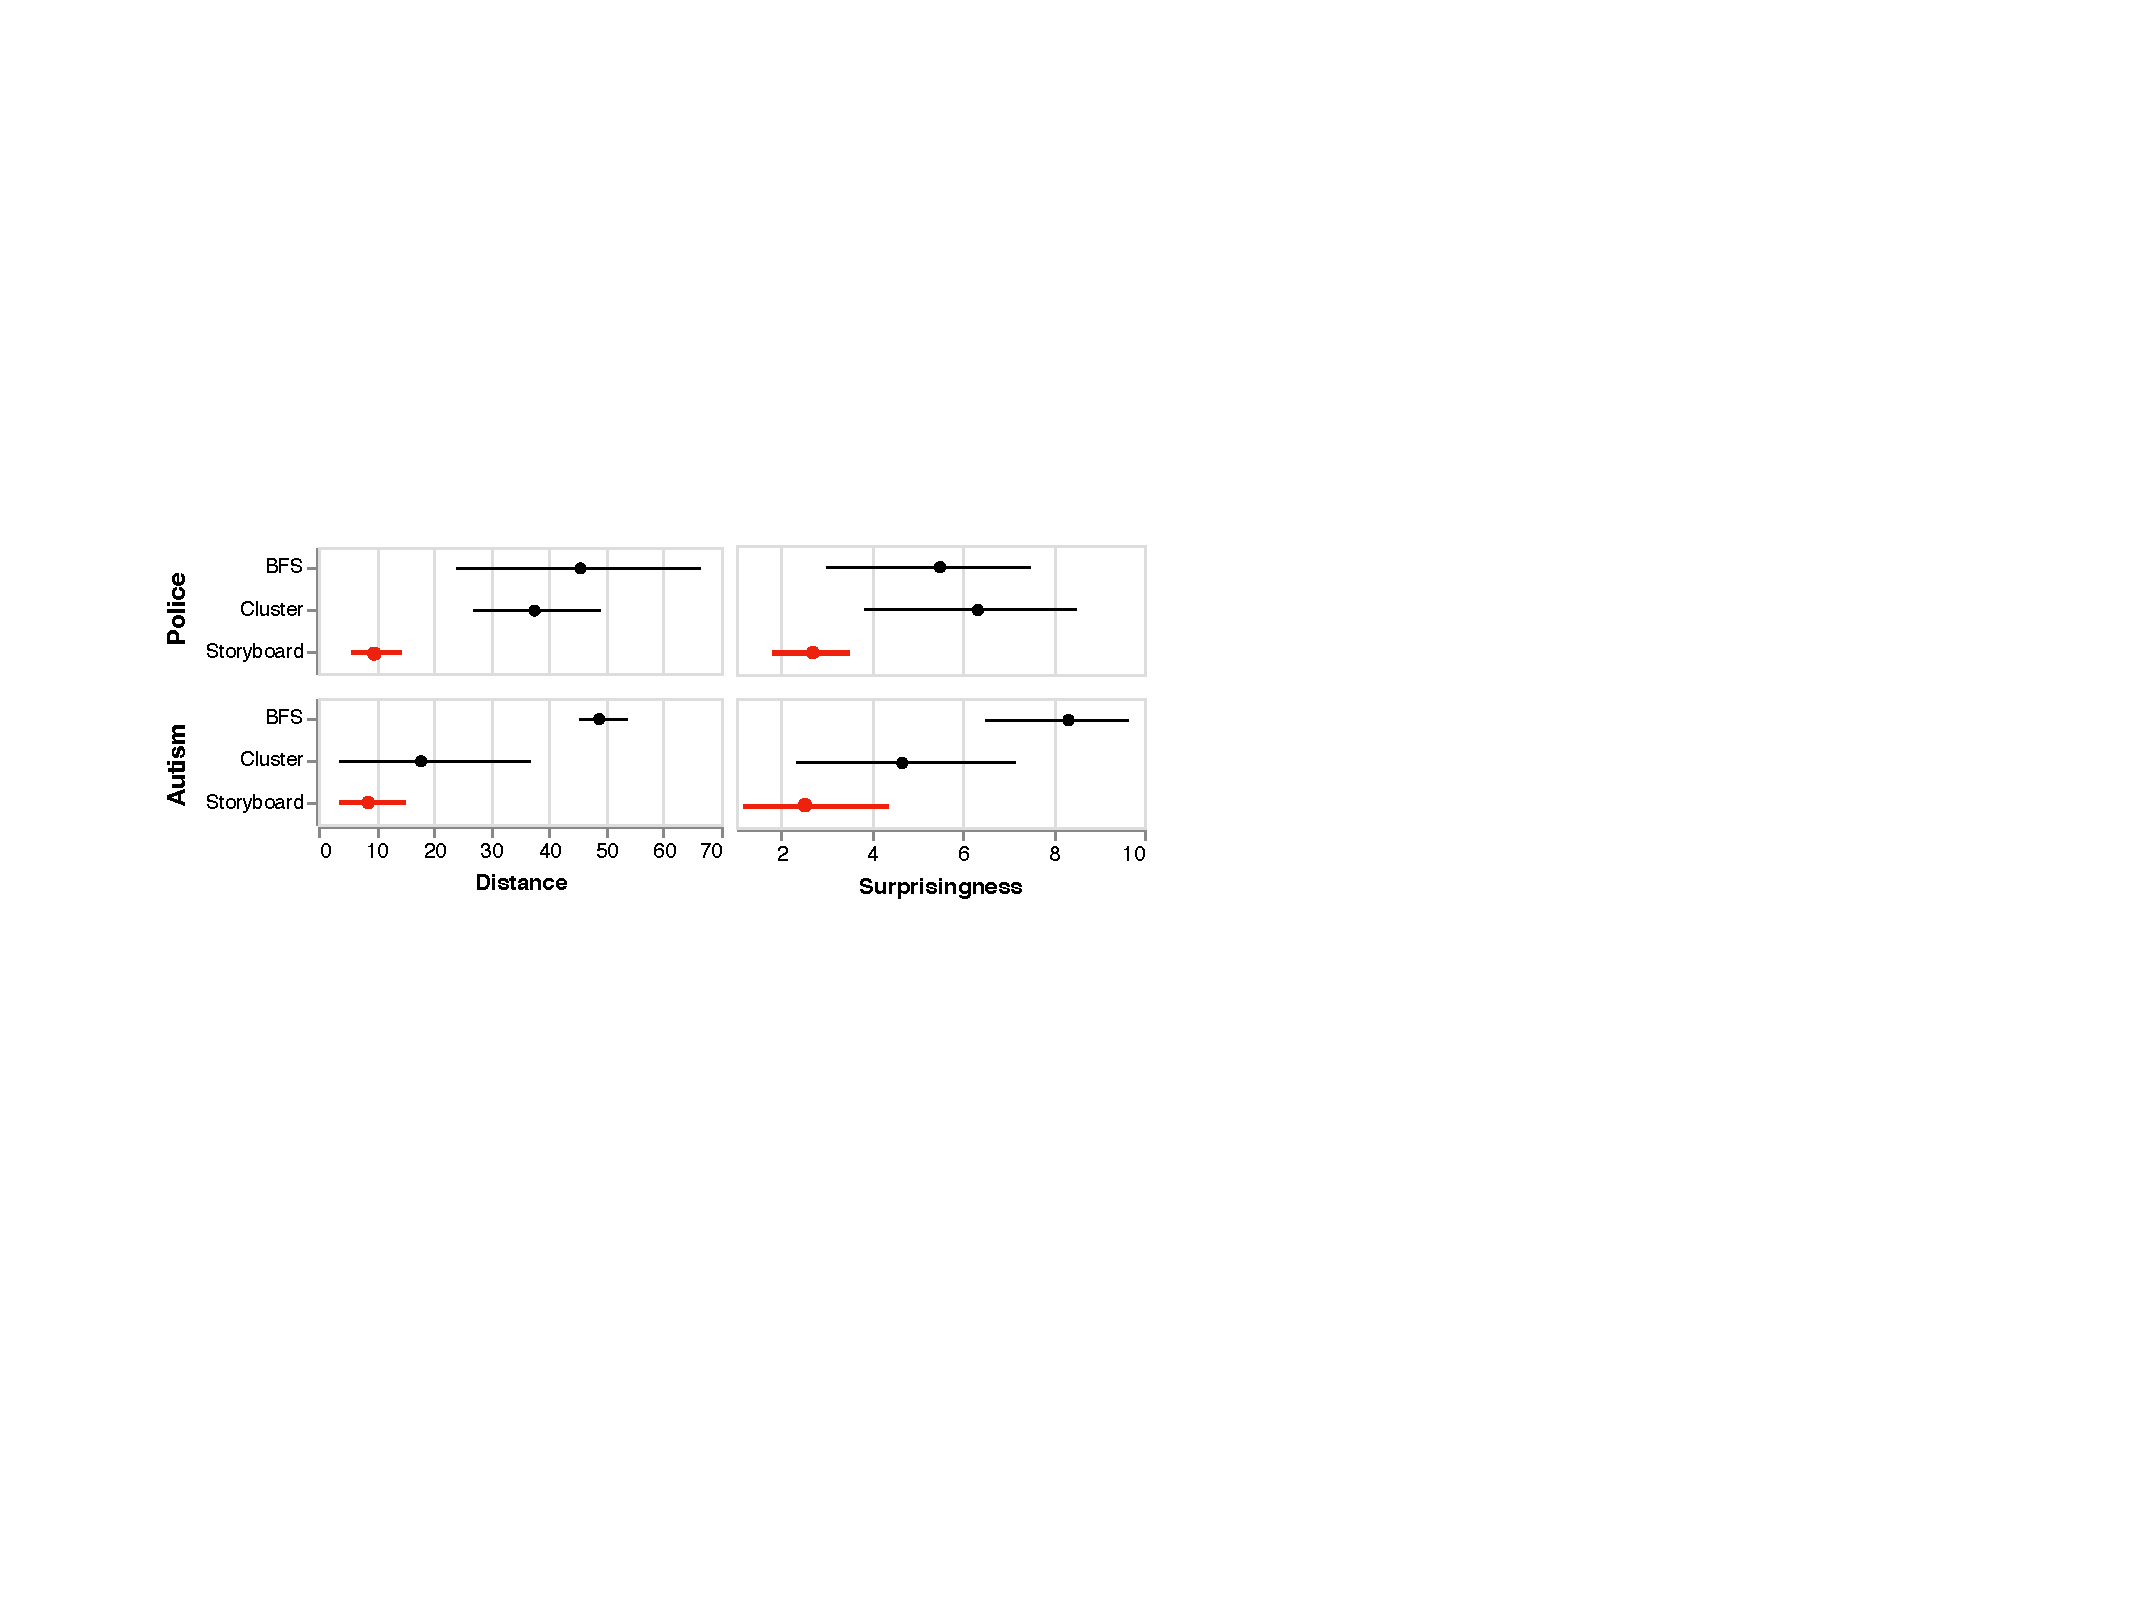
\includegraphics[width=\linewidth]{figures/prediction_surprisingness_distance.pdf}
\caption{Left: Euclidean distance between predicted and ground truth. In general, predictions made using \system is closer to the ground truth. Right: Surprisingness rating reported by users after seeing the actual visualizations on a Likert scale of 10. \system participants had a more accurate mental model of the unseen visualization and therefore reported less surprise than compared to the baseline.}
\label{fig:distance}
\end{figure}
% \par \system\ did not perform as well compared to the baselines for the Autism deep prediction task. One possible reason for this is due to the fact that the shallow and deep prediction tasks for the Autism dataset were correlated. Therefore, after learning about the insights that answering 1 on question 9 results in a very high probability for an autism diagnosis, some participants made use of that information when tackling the subsequent deep prediction task. By discussing with the baseline participants on how they have obtained the prediction estimates, they described how surprised they were by the finding in the shallow prediction and therefore adjusted the autism diagnosed values to be higher to compensate for their mistake in the subsequent deep prediction task.
\par We also compute the variance of participants' predictions across the same task. In this case, low variance implies that any user who reads the dashboard is able to provide consistent predictions, whereas high variance implies that the dashboard did not convey a clear data-driven story that could guide their predictions. So instead, participants relied on different priors or guessing to form their prediction. These trends can be observed in Figure \ref{fig:actual_predictions}, where the prediction variance amongst participants who used \system\ is generally lower than the variance from the baselines.
\begin{figure}[h!]
\centering
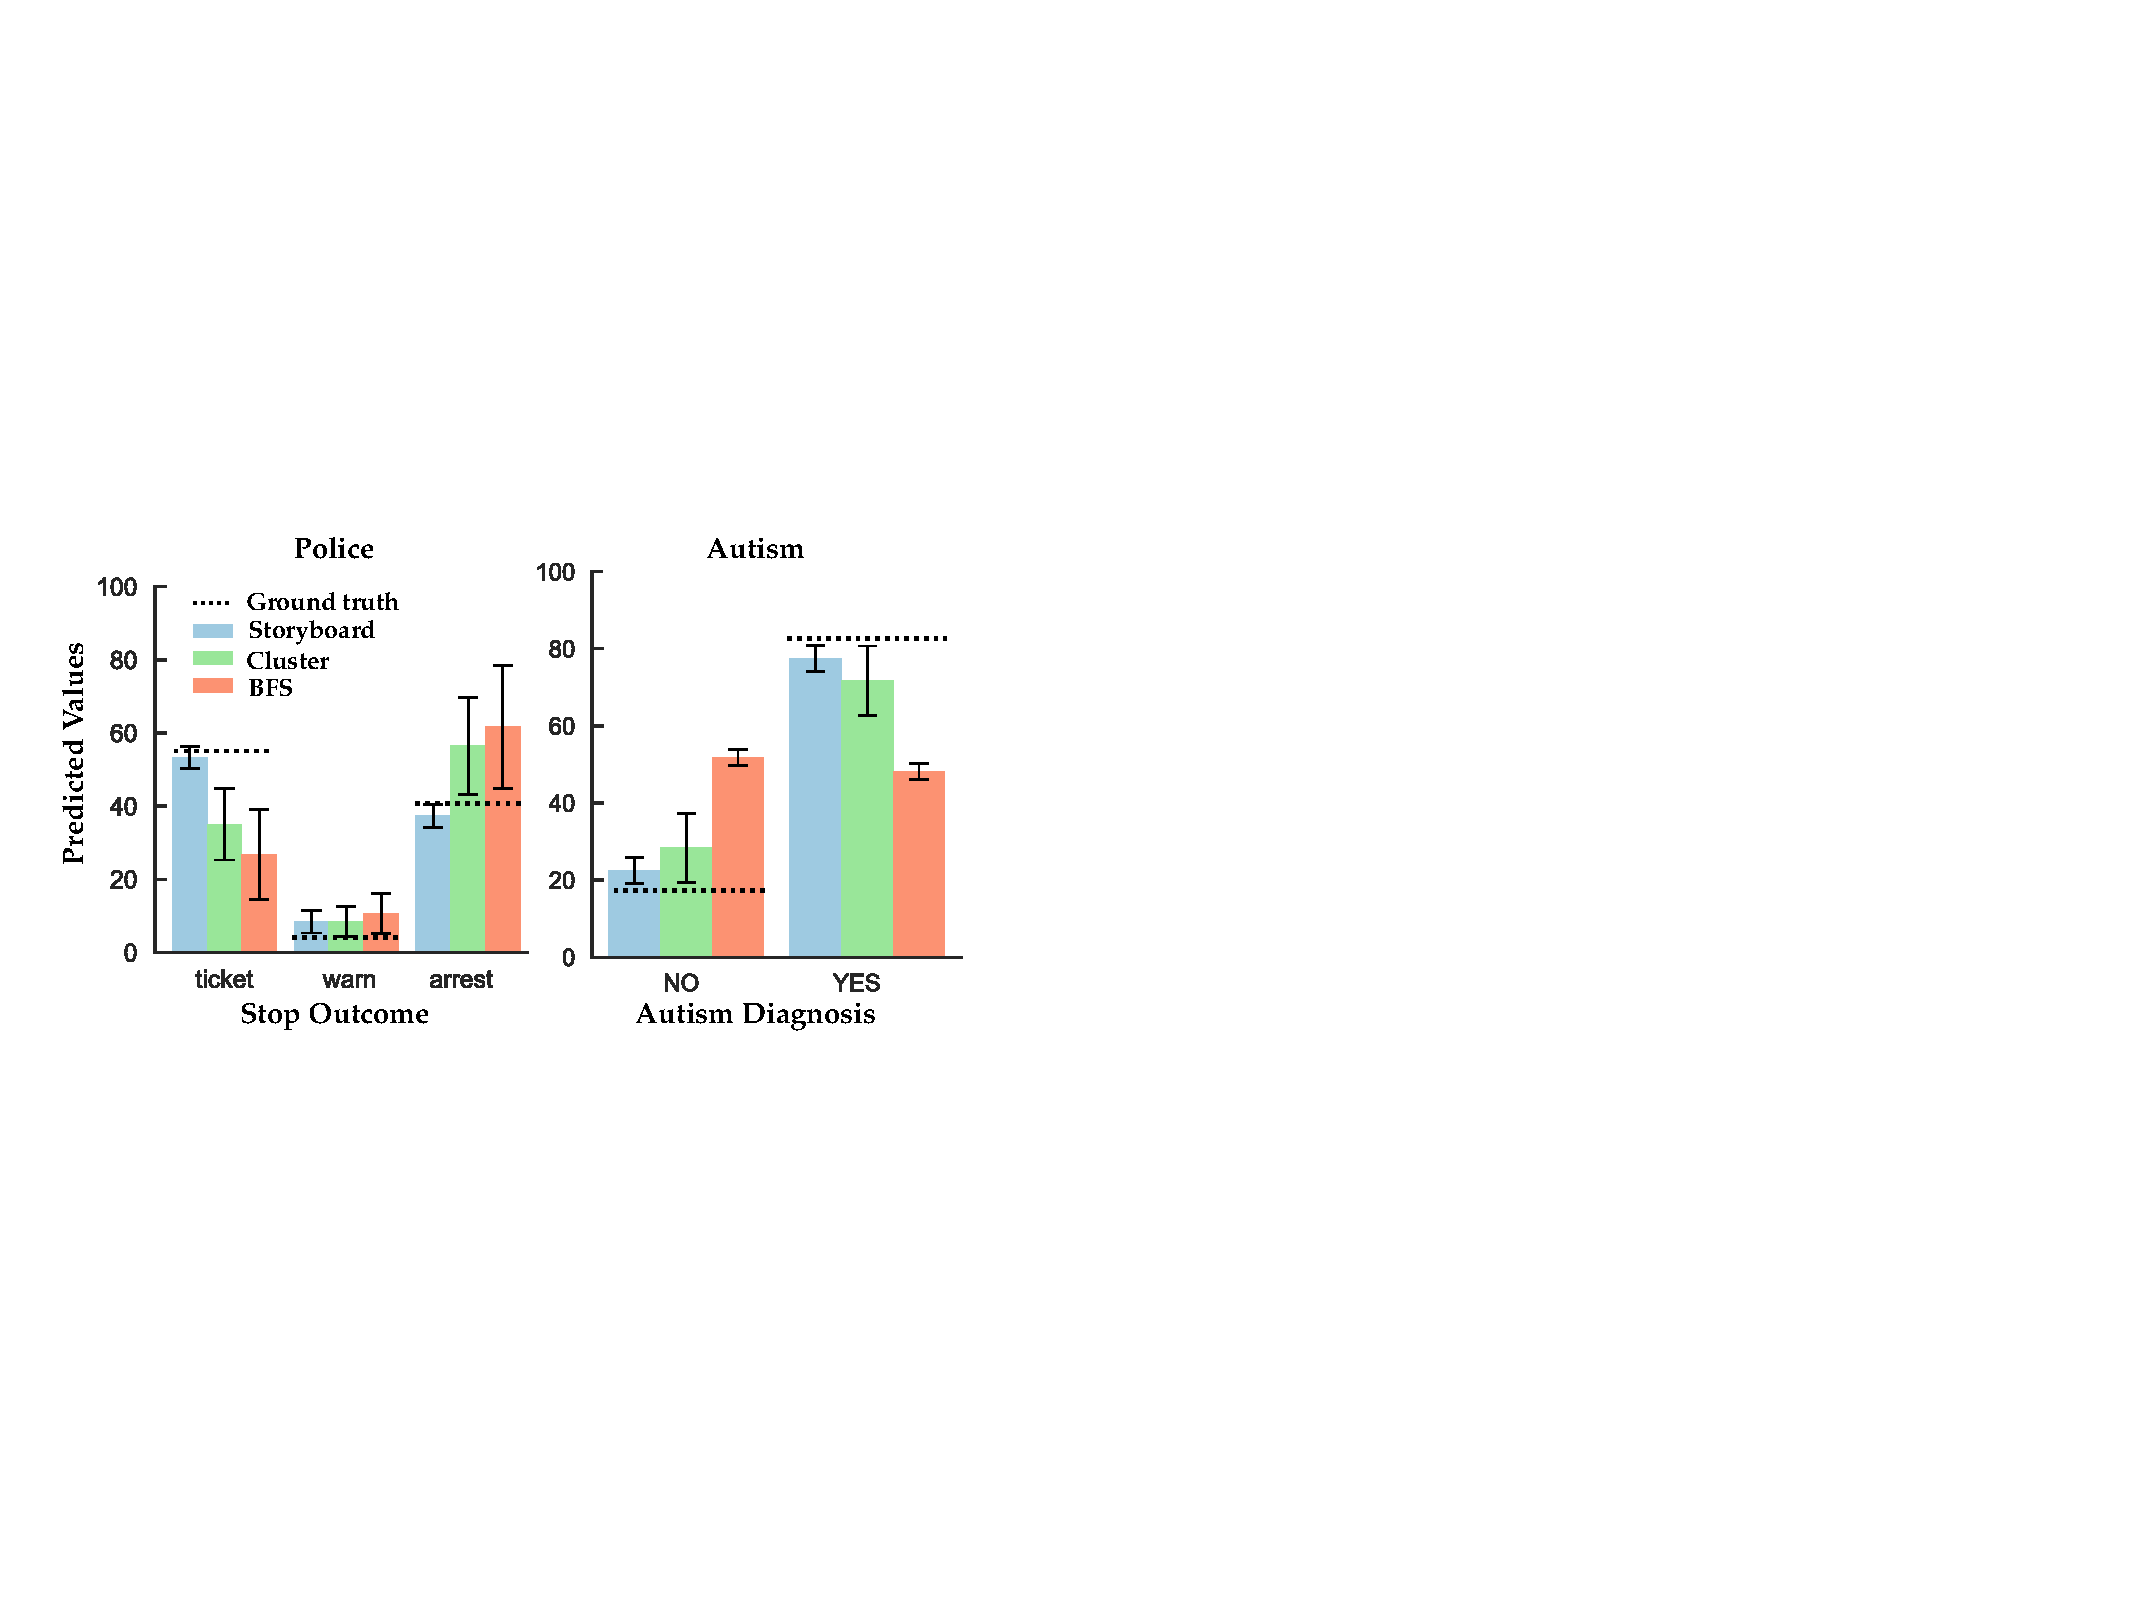
\includegraphics[width=0.8\linewidth]{figures/prediction.pdf}
\caption{Mean and variance of predicted values. Predictions based on \system exhibits lower variance (as indicated by the error bars) and great proximity to the ground truth values (dotted).}
\label{fig:actual_predictions}
\end{figure}